\documentclass[12pt]{article}
 \usepackage[margin=1in]{geometry} 
\usepackage{amsmath}
\usepackage[utf8]{inputenc}
%\usepackage[ utf8 ]{inputenc}
\usepackage[magyar]{babel}
\newcommand{\N}{\mathbb{N}}
\newcommand{\Z}{\mathbb{Z}}
\usepackage{t1enc}
\usepackage{listings}
\usepackage{placeins}
\usepackage{caption}
\usepackage{color}

\usepackage{graphicx}
\usepackage{placeins}
\usepackage{float}
\usepackage{subfigure}

\usepackage{indentfirst}
\usepackage[utf8]{inputenc}
\usepackage[T1]{fontenc}
\title{Véletlen fizikai folyamatok, hetedik házi feladat}
\author{Horváth Bendegúz}




\begin{document}
\lstset{frame=tb,
  language=python,
  aboveskip=3mm,
  belowskip=3mm,
  showstringspaces=false,
  columns=flexible,
  basicstyle={\small\ttfamily},
  numbers=none,
  numberstyle=\tiny\color{gray},
  keywordstyle=\color{blue},
  commentstyle=\color{dkgreen},
  stringstyle=\color{mauve},
  breaklines=true,
  breakatwhitespace=true,
  tabsize=3
}

\maketitle
\section*{Szimuláció}

A szimulációt \texttt{python} nyelven valósítottam meg. Előszőr importáltam a szükséges csomagokat, kiírtam a \texttt{betaJ} listába a saját $\beta J$ változóimat, majd elkészítettem egy Energia függvényt, ami a listaként megadott spinláncból kiszámolja az enerrgiát, $J$ faktor nélkül. 
\begin{lstlisting}
%pylab inline
q = 0
betaJ = [0.14, 0.28, 0.56, 1.15]

def E(spins):
    s = 0
    for i in range(1, len(spins)):
        s = s+ spins[i-1]*spins[i]
    E = -s
    return E
\end{lstlisting}
Ezek után létrehoztam egy \texttt{dE} függvényt, ami a $\Delta E$-t számolja ki, majd a \texttt{simulationStep} függgvényt, ami egy szimulációs lépésnek felel meg.
\begin{lstlisting}
def dE(s0,s1, s2):
    return 2*s1*(s0+s2)
def simulationStep(s, N, betaJ):
    rand = random.randint(0, N) 
    if rand ==0:
        s1 = s[rand]
        s0 = s[N-1]
        s2 = s[rand+1]
    if rand == N-1:
        s1 = s[rand]
        s0 = s[rand-1]
        s2 = s[0]
    else:
        s0 = s[rand-1]
        s1 = s[rand]
        s2 = s[rand+1]
    if dE(s0, s1, s2) <0:
        s[rand]= -s[rand]
        return s
    elif dE(s0, s1, s2) == 0:
        P = random.random()
        if P< 0.5:
            s[rand]= -s[rand]
            return s
        else:
            return s
    else: 
        P = random.random()
        if P < exp(-betaJ*dE(s0, s1, s2)):
            s[rand] = -s[rand]
            return s
        else:
            return s
        
\end{lstlisting}
Egy szimuláció során $t =1000$-ig néztem, így $1000\cdot 100 = t\cdot N$ lépés volt. Egy $\beta J$-re több mérést is megnéztem. A végeredménynek a mérések átlagát veszem, hibának a mérések szórását. Az eredmények a következőnek adódtak: 

\begin{center}
\begin{tabular}{|c|c|c|c|c|}\hline
mérés & $\beta J$ & m& $ \langle m \rangle $ & $\sigma^2_m$ \\ \hline
0&0.14& 0.3& 0.0035& 0.01287\\ \hline
1&0.14&0.08&-0.00649&0.0126422\\ \hline
2&0.14&-0.14&0.00288& 0.0127007\\ \hline
3& 0.14&-0.04&0.0081& 0.01132\\ \hline
4&0.14&0.02&0.00566&0.01295 \\ \hline
átlag& 0.14&$0.044\pm0.0217$&$0.00273\pm(2.460\cdot 10^{-5})$&$ 0.0125\pm(3.62\cdot 10^{-7})$\\ \hline
\end{tabular}
\end{center}

\begin{center}
\begin{tabular}{|c|c|c|c|c|}\hline
mérés & $\beta J$ & m& $ \langle m \rangle $ & $\sigma^2_m$ \\ \hline
0&0.28&0.34& -0.003&0.0183\\ \hline
1&0.28& -0.02&0.0055&0.0200\\ \hline
2&0.28&0.04&-0.0037&0.01732\\ \hline
3&0.28&0.02&0.0053&0.01608\\ \hline
4&0.28&-0.06&0.00133&0.01585\\ \hline
átlag&0.28&$0.095\pm0.02$&$0.0010\pm(1.53\cdot 10^{-5})$&$0.0.0175\pm(2.351\cdot 10^{-6})$\\ \hline
\end{tabular}
\end{center}

\begin{center}
\begin{tabular}{|c|c|c|c|c|}\hline
mérés & $\beta J$ & m& $ \langle m \rangle $ & $\sigma^2_m$ \\ \hline
0&0.56&0.26&0.00393&0.02725 \\ \hline
1&0.56&0.16&0.17157&0.02941 \\ \hline
2&0.56&0.06&-0.004066&0.03215 \\ \hline
3&0.56&-0.02&0.00613&0.02872 \\ \hline
4&0.56& 0.22&-0.0195& 0.030677 \\ \hline
átlag&0.56&$0.079\pm0.01$&$0.00122\pm(1.65\cdot 10^{-3})$&$0.02964\pm(2.797\cdot 10^{-6})$\\ \hline
\end{tabular}
\end{center}


\begin{center}
\begin{tabular}{|c|c|c|c|c|}\hline
mérés & $\beta J$ & m& $ \langle m \rangle $ & $\sigma^2_m$ \\ \hline
0&1.15&0.1&-0.07922&0.1089 \\ \hline
1&1.15&0.4&0.01964&0.06454\\ \hline
2&1.15&-0.04& -0.1458&0.10169 \\ \hline
3& 1.15&0.34&-0.005755&0.11115 \\ \hline
4&1.15&-0.36&0.15794&0.06074\\ \hline
átlag&1.15&$0.2\pm0.031$&$0.000172\pm(0.01158)$&$0.089\pm(4.8\cdot 10^{-4})$\\ \hline
\end{tabular}
\end{center}

\begin{figure}[H]
\centering
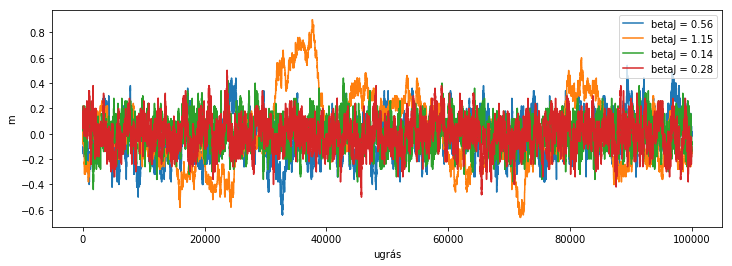
\includegraphics[width = 150mm]{four}

\caption{A $m$ értékeinek változása ugrásonként, különböző $\beta J$ értékekkel}
\label{fig: elso}
\end{figure}

A \ref{fig: elso} ábrán látszik, ami a táblázatadatokban is, hogy a $\beta J$ értékének növelésével a szórás nő. Megvizsgálva a többi mennyiséget nem kapunk ilyen egyértelmű össszefüggést.

\begin{figure}[H]
\centering     
\subfigure[]{\label{fig:a}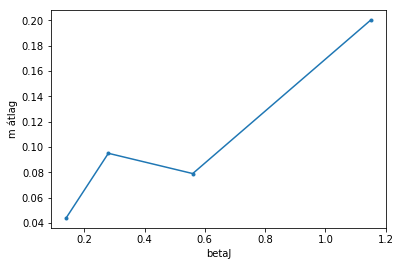
\includegraphics[width=50mm, height = 35mm]{one}}
\subfigure[]{\label{fig:b}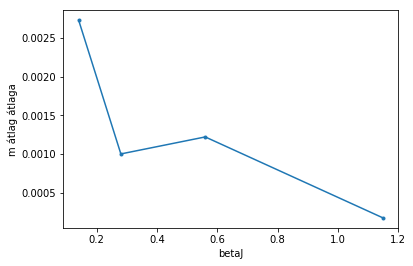
\includegraphics[width=50mm, height = 35mm]{two}}
\subfigure[]{\label{fig:b}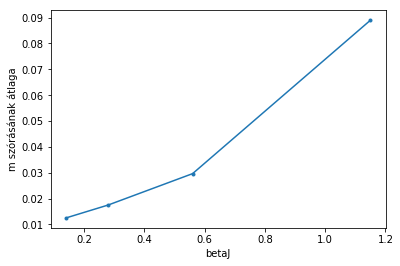
\includegraphics[width = 50 mm,height=35mm]{three}}

\caption{(a) az egyes csúcsokhoz tartozó kapcsolatok száma (b) $\langle m\rangle$ átlagának változása,(c) $\sigma_m$ átlagának változása a $\beta J$ értékének függvényében.}
\label{fig: k}
\end{figure}


\end{document}